\chapter{Systém PerfEval}

\section{Popis systému}

S rozborem problematiky ve druhé kapitole je možné začít řešit programátorův
problém s vyhodnocováním výkonu popsaný ve scénáři z první kapitoly.
V důsledku toho je cílem vytvořit systém, který umožní porovnávat výsledky
měření výkonu, a který bude možné používat v rámci průběžné integrace.

Když už jsou známy požadavky na aplikaci, tak je možné ji začít navrhovat.
V této kapitole jsou popsané úvahy a rozhodnuté, které byly v průběhu vývoje
provedeny. Tyto úvahy a rozhodnutí vedly k tomu, že vyvinutý systém PerfEval je konzolová aplikace,
jejíž činnost je ovládaná příkazy a~parametry na~příkazové řádce.
Příkazy umožňují inicializovat systém, přidávat nové výsledky měření a~vyhodnocovat mezi sebou výsledky
měření dvou verzí.

\section{Rozbor alternativ v řešení}
Při~vývoji systému PerfEval došlo k~několika rozhodnutím, které výrazně ovlivnily jeho fungování a~architekturu.
Nejdůležitější rozhodnutí, která byla v~průběhu vývoje provedena, jsou v~následujících částech podrobně vysvětlena.

\subsection{Spouštění testů systémem PerfEval}
V~počátku vývoje bylo nutné se~rozhodnout, jakým způsobem bude systém přijímat a~zpracovávat výsledky testů.
V~úvahu přicházela varianta, že~uživatel provede měření výkonu sám, a~druhá varianta, že~uživatel systému
vysvětlí, jakým způsobem se~testování výkonu spouští. Pokud by byla zvolena varianta, kdy PerfEval spouští testy
sám, tak by bylo nutné nalézt dostatečně univerzální způsob spouštění testů.

Aplikace a~benchmarky pro měření výkonu mohou být jak konzolové, tak grafické aplikace. Pokud by PerfEval měl
měření provádět sám, tak by téměř určitě nebyl schopen pracovat s~grafickými aplikacemi, ale byl by schopen
spouštět programy s~parametry na~příkazové řádce.

Dále by bylo nutné vysvětlit, jak vypadá výstup spouštěných testů. Když pomineme formát, tak je nutné zjistit,
kam program, který provádí měření výsledky ukládá. Benchmarkovací systém BenchmarkDotNet například vypisuje
výsledky měření v podobě tabulky na standardní výstup a~zároveň ukládá strojově čitelné výsledky do~speciálního
k~tomu určeného adresáře.

Nakonec by to vypadalo tak, že při inicializaci systému uživatel zadá, jak spustit test výkonu a~kam se uloží výsledek.
Tímto způsobem by došlo k~tomu, že~PerfEval by začal určovat, jak mají vypadat programy, jejichž výstupy přijímá.
Na druhou stranu použití stávajícího řešení tyto nevýhody nemá. Jediné, co~musí uživatel zajistit, je, že~jeho
způsob měření zvládne uložit výsledek do~souboru, který PerfEval umí zpracovat.

Stávající řešení je tedy složitější v tom, že~uživatel musí testování výkonu spouštět sám. Poté, co~spustí testování
výkonu a~dostane soubor s~výsledky, jej přidá do databáze výsledků systému PerfEval a~poté spustí PerfEval s~příkazem evaluate
pro porovnání výsledků testování výkonu. Kdyby se použila varianta s~tím, že si PerfEval spouští testy sám, tak
by uživatel testování a~porovnání výkonu zvládl jedním spuštěním aplikace.

\subsection{Použité statistické metody}
Pro porovnání dvou výsledků měření se používají statistické metody. Statistické metody se používají ke zjištění,
jestli výsledky měření považované za~náhodné veličiny mají stejné rozdělení, popřípadě jestli je vzorků dostatečné množství.
V~systému PerfEval jsou implementovány statistické metody bootstrap a~t-test.

Pomocí bootstrapu dochází k~iluzi, že vzorků je mnohem více, než je jich ve skutečnosti změřeno. Protože měření vzorků
je samo o~sobě dlouhotrvající proces, tak se použití této statistické metody vyplatí. Bootstrap má ale tu nevýhodu, že jeho výpočet
může oproti prostému zkoumání vzorků trvat delší dobu.

t-test je tedy možné zvolit namísto bootstrapu kvůli tomu, že je rychlejší. Oproti náhodnému vybírání vzorků z~dvoudimenzionální sady
dat, kterým vzorky odpovídají, dochází k~pouhému dosazení hodnot do vzorce.

Uživatel by se tedy při volbě testu měl rozhodovat na základě toho kolik má změřených vzorků a~kolik má času na porovnání
výsledků měření. Pokud má uživatel naměřených vzorků málo a větší množství času k vyhodnocení doporučuje se použít bootstrap.
Pokud má uživatel větší množství vzorků a~málo času je pro něho lepší použít t-test.

\subsection{Rozpoznání formátu výsledků měření}

Systém, který porovnává výsledky měření výkonu, by měl mít informace o~tom v~jakém formátu jsou data uložena
a~který benchmarkovací framework je vytvořil. Podle použitého frameworku a~formátu je totiž možné výsledky
měření zpracovat pomocí programu a~transformovat data o~měření tak, aby jim systém rozuměl.
Problém je tedy jak se systém dozví o~tomto formátu a~o~použitém frameworku.

Nejpříjemnější řešení pro uživatele by bylo, že by systém sám přišel na to, který framework a~formát je použitý.
Uživatel by totiž nemusel vědět pomocí jakého frameworku a~v~jakém formátu data ukládá. Pro systém by však mohl
být problém různé frameworky rozlišit.

Při rozlišování by se totiž musel podívat do~dat uložených v souboru
a~na~základě obsahu určit o~jaký formát a~framework se jedná. Správné určení frameworku a~formátu by bylo zásadní pro
správnou reprezentaci dat. Samotné rozlišování frameworků a~formátu by bylo obtížné, protože soubory s~výsledky
měření obsahují podobná data a~položky, ale hierarchie struktur ve~kterých jsou uloženy jsou různé.
Při následném rozlišování většího množství formátů a~frameworků by tedy systém automatického rozpoznávání
začal být příliš komplikovaný, aby si zachoval přesnost.

Docházelo by také k~dvojímu čtení souboru z~paměti. První čtení souboru by sloužilo k rozpoznání formátu,
aby systém zjistil, jak má data ze souboru zpracovávat. Při druhém čtení souboru by již transformoval data
tak, aby jim rozuměla vyhodnocovací část systému.

PerfEval tedy řeší tento problém tak, že uživatel při inicializaci zadá jméno jednoho z~dostupných parserů.
Předpokládá se tedy, že pokud uživatel používá výkonnostní testy, tak framework a~výstupní formát je shodný.
Pokud má PerfEval parser pro tento framework a formát dat parser, pak je schopný vyhodnocovat výsledky měření.
V~opačném případě si tento parser může uživatel doimplementovat.

Tento přístup umožňuje snazší implementaci nových parserů. Není totiž nutné k těmto parserům implementovat
také sadu pravidel, kdy má být použitý. Uživatele tento přístup omezuje v tom, že musí znát framework a~formát
ve~kterém se výsledky měření nachází. Protože psaní výkonnostních testů není jednoduché, tak lze předpokládat,
že uživatel je dostatečně zkušený, aby tuto znalost měl.

\subsection{Kdy zpracovávat naměřená data?}

Systém musí v~některém bodě výpočtu zpracovat data z~měření. Existuje několik možností, kdy
je možné toto zpracování do formátu, kterému bude rozumět, udělat. Je možné buď zpracovat
data ihned po tom, co se systém dozví o~jejich existenci, nebo až těsně před vyhodnocováním.

Pokud by se data zpracovávala hned po tom, co se o nich systém dozví, tak to nutně neznamená,
že již má proběhnout vyhodnocování. Je tedy nutné zvolit nějaký formát do kterého zpracovaná data
uložit. Při vyhodnocení by se pak data z tohoto formátu musela opět zpracovat. Tento způsob
zpracování dat by měl význam pouze v~případě, že by první předzpracování vedlo k~velkému
zrychlení druhého zpracování. Zároveň by toto řešení vedlo k dvojímu ukládání dat, protože
by někde byl uložený původní výsledek měření v původním formátu, a také soubor se předzpracovanými
výsledky měření, který by obsahoval data se stejným významem.

Výše zmíněné nevýhody vedly k tomu, že systém zpracovává data z~původního formátu těsně před
vyhodnocováním. Podle zvoleného parseru se tedy data naparsují těsně před vyhodnocením ze~souborů,
které vygeneroval přímo framework pro měření výkonu.

\subsection{Jak přistupovat k naměřeným datům?}

Systém, který porovnává výsledky měření, by měl mít nějaké informace o~tom, k~jaké verzi se měření vztahuje, nebo kde
se soubor s~výsledky nachází. Proto bylo při vývoji nutné se zamyslet nad tím, jakými způsoby lze tyto informace získat a~spravovat.
Systém PerfEval potřebuje o~výsledcích měření vědět, kde jsou uloženy a~ke~které verzi softwaru bylo měření provedeno.

První zvažovaná varianta byla, že by existovala složka, do~které by uživatel vkládal výsledky měření do~adresáře určeného
systémem PerfEval, nebo do~adresáře zadaného při inicializaci systému. Po~každém měření by tedy uživatel výsledek pouze
vložil do~správné složky a~o~nic víc by se nemusel starat.

Toto řešení má několik nevýhod. Omezuje uživatele v~tom, jak musí výsledky testů ukládat. Dále by se špatně určovalo, ke~
které verzi bylo měření provedeno, protože toto se ve~výsledcích měření běžnými frameworky neudává. Pravděpodobně by proto
vznikla hierarchie v tomto adresáři a~uživatel by například pomocí pojmenovávání složek určoval, ke~které verzi se měření vztahuje.

Celkově tedy tento způsob poskytuje jednoduché zjištění, kde se výsledek testu nachází. Je to pevně dané. Není ale možné jednoduše
zjistit verzi, protože je nutné projít adresářovou strukturu, což může být při velkém množství dat pomalé.

Druhé uvažované řešení bylo vylepšení prvního řešení o~cache a sledování času modifikace adresářů. Verze se totiž dobře určují,
ale špatně dohledávají. Nicméně by se pravděpodobně používání některých verzí k~porovnání opakovalo častěji než u~jiných.
Zároveň pokud by nejnovější verze nebyla v cache, tak by se dohledávala na základě nejmladšího data změny adresáře
v~adresáři s~výsledky měření. Cache by byla tvořena posledními několika desítkami záznamů s~cestou k~výsledkům měření a~verzí.

Toto řešení má ale podobné nevýhody jako první. V~případě, že se verze porovnává poprvé, tak záznamy o~ní jistě nejsou v~cache
a~musí se prohledat adresářová struktura. Pokud je poslední úprava cache starší než nejnovější úprava nějakého podadresáře v~adresáři
s~výsledky měření, tak je nutné tuto část adresářové struktury projít. V~procházené části adresářové struktury je vždy nutné prozkoumat
zdali se jedná o~soubor verze, která je v cache, a~tak by se do ní měl přidat záznam o~tomto souboru. Popsaná práce s~cache měla
za~následek poslední uvažované řešení, kde již nezáleží na tom, kde jsou uložené výsledky měření. Jediné, co budeme předpokládat, je,
že uživatel soubory s~výsledky měření nepřesouvá.

Poslední uvažované řešení je strukturované ukládání metadat o~výsledcích měření. Využije se databáze o~jedné tabulce, kde
je uvedena cesta k~výsledku měření a~verze ke které byl výsledek změřen. Uživatel do~systému nahlásí, že má nový výsledek
měření, kde je uložen, a~k~jaké verzi softwaru je měření provedeno. Systém si tato data pouze poznamená do~databáze. Při
vyhodnocení pak pomocí databázových dotazů nalezen snadno všechny soubory s~výsledky měření k~potřebné verzi.

Toto řešení poskytuje jak rychlé vkládání nových výsledků, tak rychlé vyhledávání výsledků měření k~dané verzi.

\subsection{Formát výstupu}

Při volbě formátu v~jakém se budou výsledky výkonnostních testů prezentovat je nutné se zamyslet nad tím, kdo je bude číst a~zpracovávat.
Výsledky vyhodnocení bude zpracovávat zejména člověk a~průběžná integrace v~rámci verzovacího nástroje Git.

Pro člověka je čitelný formát zpracovaných dat tabulka s údaji o~tom, který test prošel a~který ne.
Jeden z~výstupních formátu systému PerfEval je takováto tabulka na příkazové řádce.

\section{Architektura systému PerfEval}

\subsection{Průběh vyhodnocování}

Na následujícím obrázku je k~vidění architektura části systému kolem třídy EvaluateCLICommand, která zajišťuje
průběh vyhodnocování testů výkonu.

\begin{figure}[!ht]
    \centering
    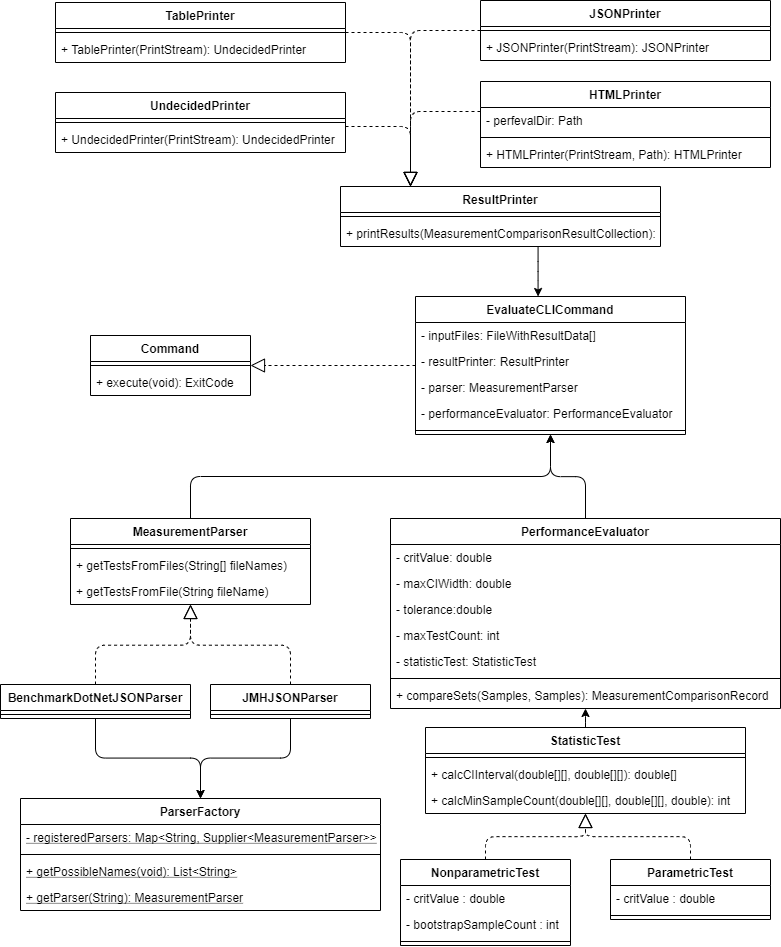
\includegraphics[width=0.92\textwidth]{../img/perfeval_evaluate.png}
    \caption{Objektový návrh části PerfEvalu pro porovnávání výsledků měření}
\end{figure}

Po~zpracování příkazové řádky dostane instance EvaluateCLICommand informace
o~souborech se kterými bude pracovat. Při~konstrukci dostane správné implementace ResultPrinter,
MeasurementParser a~instanci třídy PerformanceEvaluator se správnou instancí StatisticTest.

Hlavní funkcionalitu pro~vyhodnocování poskytuje třída EvaluateCLICommand. Celý úkol vyhodnocování výkonu
byl rozdělen do~tří oddělených kroků.

Jako první dojde k~naparsování výsledků měření dvou porovnávaných verzí. Parsování probíhá pomocí
implementace rozhraní MeasurementParser, který umí naparsovat potřebný formát výsledků měření, které
se budou porovnávat. Výsledkem parsování vzniknou dvě instance třídy Samples, která reprezentuje vzorky
výsledků měření.

Následně se tyto dvě instance porovnají pomocí metody compareSets na~třídě PerformanceEvaluator. Instance třídy
PerformanceEvaluator k~porovnání dvou instancí Samples využívá implementace rozhraní StatisticTest. Konkrétně
tato implementace rozhoduje o~tom, jaký statistický test se při porovnávání vzorků použije.

Statistický test, který implementuje rozhraní StatisticTest, musí mít metody calcCIInterval a~calcMinSampleCount.
Metoda calcCIInterval vrací intervalový odhad rozdílu náhodných veličin, které jsou reprezentovány konkrétními
naměřenými vzorky.

Pokud tento interval neobsahuje nulu, pak lze s~požadovanou přesností a~pravděpodobností usuzovat,
že rozdělení náhodných veličin jsou různá. Pokud jsou rozdělení různá, pak se jako kladný výsledek testu připouští
zlepšení výkonu, nebo pokud je nový průměr v dané toleranci.

Pokud interval obsahuje nulu, tak je vyhodnocení výsledku testu výkonu složitější. Pokud je interval spolehlivosti
dostatečně úzký, tak považujeme rozdělení náhodných veličin za stejná a~test výkonu dopadl kladně. Pokud interval
spolehlivosti není dostatečně úzký, tak test výkonu neprošel. Následně se pomocí metody calcMinSampleCount určí
kolik měření by bylo potřeba, aby byl interval spolehlivosti dostatečně úzký. Spočtený počet vzorků s~informací o~tom,
zdali je, nebo není možné je změřit, bude přidán k~výsledkům porovnávání.

Posledním krokem při vyhodnocování je zavolání metody printResults na~implementaci rozhraní ResultPrinter. Tato metoda
vypíše instanci MeasurementComparisonResultCollection, která reprezentuje všechny výsledky jednotlivých testů výkonu.
Po~vypsání výsledků požadovaným způsobem dle dodané implementace ResultPrinter se nastaví správný exit kód. V~případě,
že všechny testy dopadly kladně, pak bude exit kód 0. V~případě, že alespoň v~jednom případě došlo ke~zhoršení, pak bude
exit kód 1. V~případě, že dojde k~nějaké výjimce, tak exit kód bude větší než 100. Touto výjimkou může být například
neexistence některého ze~souborů s~naměřenými výsledky v~důsledku jeho smazání, nebo přesunutí.

\subsection{Inicializace systému PerfEval}

Před použitím systému PerfEval k~vyhodnocování je nutné jej inicializovat. Inicializace umí rozpoznat zdali se nachází
v~kořenovém adresáři Git repozitáře. Rozpoznávání probíhá tak, že se hledá soubor s názvem .git.

Inicializace probíhá tak, že se zjistí přítomnost .git souboru. Z~příkazové řádky se zjistí jaký parser (implementace
třídy MeasurementParser) pro~naměřené hodnoty se bude používat. Vyrobí výchozí konfigurace. Do~výchozí konfigurace
se dodají informace o~git repositáři a~o~parseru. Nakonec se vyrobí složka se v adresáři, kde uživatel program spustil
vyrobí složka .performance a~v~ní soubory .gitignore a~config.ini. Soubor config.ini obsahuje konfiguraci systému PerfEval
pro~jeden projekt jehož výkon mezi verzemi se bude porovnávat.

\begin{figure}[!ht]
    \centering
    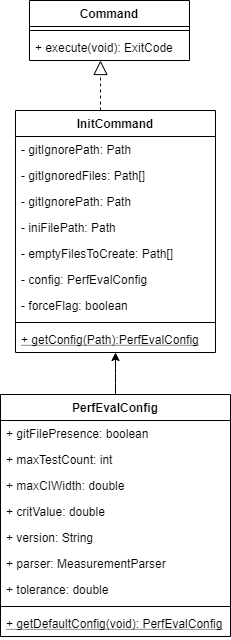
\includegraphics[height=0.5\textheight]{../img/perfeval_init.png}
    \caption{Objektový návrh části PerfEvalu pro inicializaci}
\end{figure}

Z~obrázku je patrné, že třída InitCommand úzce spolupracuje s~třídou PerfEvalConfig. Třída PerfEvalConfig reprezentuje
obsah souboru config.ini. Provedení metody execute na~třídě InitCommand provede inicializaci systému PerfEval výše
zmíněným způsobem.

\subsection{Přidávání nových výsledků testů}

Uživatel musí každý výsledek měření výkonu zaznamenat do~systému PerfEval. Pokud výsledek měření zaznamenán, nebude s~ním
PerfEval vůbec pracovat. Přidávat je možné soubory samostatně, nebo z~adresáře. Při~přidávání souborů z~adresáře budou
přidány všechny soubory a~to i~soubory zanořené ve~vnitřních adresářích zadaného adresáře.

\begin{figure}[!ht]
    \centering
    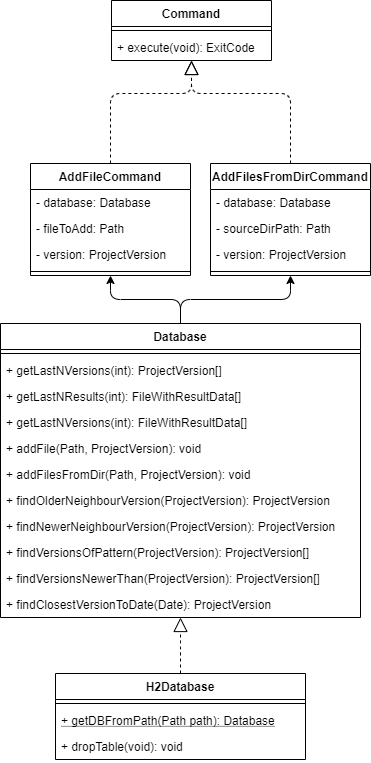
\includegraphics[height=0.5\textheight]{../img/perfeval_h2db.png}
    \caption{Objektový návrh části PerfEvalu pro přidávání výsledků měření}
\end{figure}

Na obrázku je vidět, že za~oběma příkazy pro přidávání výsledků měření stojí jedna implementace rozhraní Database.
Jediná existující implementace tohoto rozhraní využívá technologie H2 databáze. Jedná se o~technologii, která umožňuje
vést si databázi lokálně v~rámci souboru a~pokládat na ní klasické SQL dotazy.

Implementace rozhraní Database pomocí technologie H2 je třída H2Database. V~rámci databáze pro jeden projekt, který
PerfEval spravuje jsou lokální soubory pro H2 databázi uloženy v adresáři .performance. Databáze pro správu dat o~výsledcích
měření má jen jednu tabulku. V~této tabulce jsou informace o~cestě k~souboru a~informace o~verzi.

